\chapter{Annexos}
\section{Codi ESP32 per transmetre trames d'àudio en protocol I2S}
\begin{lstlisting}[language=C++, basicstyle=\ttfamily\small, breaklines=true, frame=single]
// Codi ESP32 -- Font audio I2S
// Includes

    #include "SD.h"                         
    #include "driver/i2s.h"          
  
//----------------------
//----------------------
// Defines
 
//    SD Card
    #define SD_CS          5    
   
//    I2S

    #define I2S_DOUT      25    
    #define I2S_BCLK      27   
    #define I2S_LRC       26    
    #define I2S_NUM       0    

// Wav Fitxer
    #define NUM_BYTES_TO_READ_FROM_FILE 1024   

//----------------------

//----------------------
// structures and also variables
//  I2S configuration

      static const i2s_config_t i2s_config = 
      {
          .mode = (i2s_mode_t)(I2S_MODE_MASTER | I2S_MODE_TX),
          .sample_rate = 44100,                                
          .bits_per_sample = I2S_BITS_PER_SAMPLE_16BIT,
          .channel_format = I2S_CHANNEL_FMT_RIGHT_LEFT,
          .communication_format = (i2s_comm_format_t)(I2S_COMM_FORMAT_I2S | I2S_COMM_FORMAT_I2S_MSB),
          .intr_alloc_flags = ESP_INTR_FLAG_LEVEL1,             
          .dma_buf_count = 8,                           
          .dma_buf_len = 64,                                    
          .use_apll=0,
          .tx_desc_auto_clear= true, 
          .fixed_mclk=-1    
      };
    
//----------------------
// Pin configuració      
      static const i2s_pin_config_t pin_config = 
      {
          .bck_io_num = I2S_BCLK,              
          .ws_io_num = I2S_LRC,                           
          .data_out_num = I2S_DOUT,                       
          .data_in_num = I2S_PIN_NO_CHANGE                  
      };
      
      struct WavHeader_Struct
      {
          //   RIFF Section    
          char RIFFSectionID[4];    
          uint32_t Size;             
          char RiffFormat[4];         
          
          //   Format Section    
          char FormatSectionID[4];   
          uint32_t FormatSize;       
          uint16_t FormatID;         
          uint16_t NumChannels;       
          uint32_t SampleRate;        
          uint32_t ByteRate;          
          uint16_t BlockAlign;       
          uint16_t BitsPerSample;  
        
          // Data Section
          char DataSectionID[4];      
          uint32_t DataSize;       
      }WavHeader;
//------------------

//  Global Variables/objects    
    
    File WavFile;                                
    static const i2s_port_t i2s_num = I2S_NUM_0;      

//-----------------


void setup() {    
    Serial.begin(115200);                               
    SDCardInit();
    i2s_driver_install(i2s_num, &i2s_config, 0, NULL);
    i2s_set_pin(i2s_num, &pin_config);
    WavFile = SD.open("/audioprova.wav");                   
    if(WavFile==false)
      Serial.println("Could not open 'wavfile.wav'");
    else
    {
      WavFile.read((byte *) &WavHeader,44); 
      DumpWAVHeader(&WavHeader);           
      if(ValidWavData(&WavHeader))    
        i2s_set_sample_rates(i2s_num, 44100);     
    }
}


void loop()
{    
    PlayWav();                                          
}

void PlayWav()
{
  static bool ReadingFile=true;                    
  static byte Samples[NUM_BYTES_TO_READ_FROM_FILE];   
  static uint16_t BytesRead;                          

  if(ReadingFile)                                    
  {
    BytesRead=ReadFile(Samples);                   
    ReadingFile=false;             
  }
  else
    ReadingFile=FillI2SBuffer(Samples,BytesRead);    
}

uint16_t ReadFile(byte* Samples)
{
    static uint32_t BytesReadSoFar=0;                   
    uint16_t BytesToRead;                           
    
    if(BytesReadSoFar+NUM_BYTES_TO_READ_FROM_FILE>WavHeader.DataSize)  
      BytesToRead=WavHeader.DataSize-BytesReadSoFar;          
    else
      BytesToRead=NUM_BYTES_TO_READ_FROM_FILE;             
      
    WavFile.read(Samples,BytesToRead);              
    BytesReadSoFar+=BytesToRead;         
    
    if(BytesReadSoFar>=WavHeader.DataSize)   
    {
      WavFile.seek(44);                    
      BytesReadSoFar=0;                                    
    }
    return BytesToRead;             
}

bool FillI2SBuffer(byte* Samples,uint16_t BytesInBuffer)
{
    
    size_t BytesWritten;                        
    static uint16_t BufferIdx=0;      
    uint8_t* DataPtr;              
    uint16_t BytesToSend;      
    
    DataPtr=Samples+BufferIdx;                               
    BytesToSend=BytesInBuffer-BufferIdx;                     
    i2s_write(i2s_num,DataPtr,BytesToSend,&BytesWritten,1);  
    BufferIdx+=BytesWritten;                          
    
    if(BufferIdx>=BytesInBuffer)                 
    {
      BufferIdx=0; 
      return true;                             
    }
    else
      return false;     
}

void SDCardInit()
{        
    pinMode(SD_CS, OUTPUT); 
    digitalWrite(SD_CS, LOW);
    if(!SD.begin(SD_CS))
    {
        Serial.println("Error talking to SD card!");
        while(true);                  
    }
}

bool ValidWavData(WavHeader_Struct* Wav)
{
  
  if(memcmp(Wav->RIFFSectionID,"RIFF",4)!=0) 
  {    
    Serial.print("Invalid data - Not RIFF format");
    return false;        
  }
  if(memcmp(Wav->RiffFormat,"WAVE",4)!=0)
  {
    Serial.print("Invalid data - Not Wave file");
    return false;           
  }
  if(memcmp(Wav->FormatSectionID,"fmt",3)!=0) 
  {
    Serial.print("Invalid data - No format section found");
    return false;       
  }
  if(memcmp(Wav->DataSectionID,"data",4)!=0) 
  {
    Serial.print("Invalid data - data section not found");
    return false;      
  }
  if(Wav->FormatID!=1) 
  {
    Serial.print("Invalid data - format Id must be 1");
    return false;                          
  }
  if(Wav->FormatSize!=16) 
  {
    Serial.print("Invalid data - format section size must be 16.");
    return false;                          
  }
  if((Wav->NumChannels!=1)&(Wav->NumChannels!=2))
  {
    Serial.print("Invalid data - only mono or stereo permitted.");
    return false;   
  }
  if(Wav->SampleRate>48000) 
  {
    Serial.print("Invalid data - Sample rate cannot be greater than 48000");
    return false;                       
  }
  if((Wav->BitsPerSample!=8)& (Wav->BitsPerSample!=16)) 
  {
    Serial.print("Invalid data - Only 8 or 16 bits per sample permitted.");
    return false;                        
  }
  return true;
}


void DumpWAVHeader(WavHeader_Struct* Wav)
{
  if(memcmp(Wav->RIFFSectionID,"RIFF",4)!=0)
  {
    Serial.print("Not a RIFF format file - ");    
    PrintData(Wav->RIFFSectionID,4);
    return;
  } 
  if(memcmp(Wav->RiffFormat,"WAVE",4)!=0)
  {
    Serial.print("Not a WAVE file - ");  
    PrintData(Wav->RiffFormat,4);  
    return;
  }  
  if(memcmp(Wav->FormatSectionID,"fmt",3)!=0)
  {
    Serial.print("fmt ID not present - ");
    PrintData(Wav->FormatSectionID,3);      
    return;
  } 
  if(memcmp(Wav->DataSectionID,"data",4)!=0)
  {
    Serial.print("data ID not present - "); 
    PrintData(Wav->DataSectionID,4);
    return;
  }  
  Serial.print("Total size :");Serial.println(Wav->Size);
  Serial.print("Format section size :");Serial.println(Wav->FormatSize);
  Serial.print("Wave format :");Serial.println(Wav->FormatID);
  Serial.print("Channels :");Serial.println(Wav->NumChannels);
  Serial.print("Sample Rate :");Serial.println(Wav->SampleRate);
  Serial.print("Byte Rate :");Serial.println(Wav->ByteRate);
  Serial.print("Block Align :");Serial.println(Wav->BlockAlign);
  Serial.print("Bits Per Sample :");Serial.println(Wav->BitsPerSample);
  Serial.print("Data Size :");Serial.println(Wav->DataSize);
}

void PrintData(const char* Data,uint8_t NumBytes)
{
    for(uint8_t i=0;i<NumBytes;i++)
      Serial.print(Data[i]); 
      Serial.println();  
}
\end{lstlisting}

\newpage

\section{\textit{Script} del disseny de l'etapa de filtrat i sobremostreig}
\begin{lstlisting}[language=Matlab, basicstyle=\ttfamily\small, breaklines=true, frame=single]

clc; clear all;

%% Disseny Filtre CIC Interpolador
R = 16;          
M = 1;           
N = 5;          

cicInterp = dsp.CICInterpolator(R,M,N);

freqRange = linspace(0, 3, 2048);

[H, W] = freqz(cicInterp, freqRange);

gain_correction = 1/(R^N);

%% Diagrama de Bode Filtre CIC

figure(1);
tiledlayout;
nexttile;
plot(W/pi, 20*log10(gain_correction * abs(H)), 'b', 'LineWidth', 1.5);
ylim([-150 10]);
title('Filtre CIC Resposta en Freqüència');
xlabel('Freqüència Normalitzada (\times\pi rad/mostra)');
ylabel('Magnitud (dB)');

nexttile;
phaseCIC = phasez(cicInterp,freqRange);
plot(W/pi, phaseCIC, 'b', 'LineWidth', 1.5);
title('Filtre CIC Resposta en Freqüència');
xlabel('Freqüència Normalitzada (\times\pi rad/mostra)');
ylabel('Desfassament (rad)');

%% Disseny Filtre Compensació CIC

fs = 44100;
fPass = 20000;
fStop = 22050;
ast = 80;

CICCompInterp = dsp.CICCompensationInterpolator(cicInterp,...
    InterpolationFactor=2,PassbandFrequency=fPass, ...
    StopbandFrequency=fStop,StopbandAttenuation=ast, ...
    SampleRate=fs)

[H2, W2] = freqz(CICCompInterp, freqRange);

coeff_CompCIC = coeffs(CICCompInterp);
coeff_CompCIC.Numerator(77) = 1;
valors_CICComp = round(coeff_CompCIC.Numerator*power(2,17)-1);

%% Diagrama de Bode Filtre Compensació CIC

figure(2);
tiledlayout;
nexttile;
plot(W2/pi, 20*log10(abs(H2)), 'b', 'LineWidth', 1.5);
ylim([-100 20]);
title('Filtre Compensació Resposta en Freqüència');
xlabel('Freqüència Normalitzada (\times\pi rad/mostra)');
ylabel('Magnitud (dB)');

nexttile;
phaseCICComp = phasez(CICCompInterp,freqRange);
plot(W2/pi, phaseCICComp, 'b', 'LineWidth', 1.5);
title('Filtre Compensació en Freqüència');
xlabel('Freqüència Normalitzada (\times\pi rad/mostra)');
ylabel('Desfassament (rad)');

%%  Etapa de Filtrat Final

FC = dsp.FilterCascade(CICCompInterp, cicInterp);
[H3, W3] = freqz(FC, freqRange);

%% Diagrama de Bode de l'Etapa de filtrat.

figure(3);
tiledlayout;
nexttile;
plot(W3, 20*log10((gain_correction/2) * abs(H3)), 'b', 'LineWidth', 1.5);
ylim([-150 10]);
title('Etapa de Filtrat Resposta en Freqüència');
xlabel('Freqüència (Hz)');
ylabel('Magnitud (dB)');

nexttile;
phaseFC = phasez(FC,freqRange);
plot(W3, phaseFC, 'b', 'LineWidth', 1.5);
title('Etapa de Filtrat Resposta en Freqüència');
xlabel('Freqüència (Hz)');
ylabel('Desfassament (rad)');

%% Càlculs de l'Etapa de filtrat
indH = find((gain_correction/2)*abs(H3) < sqrt(1/2), 1, 'first');
slopeH = (gain_correction/2)*(abs(H3(indH)) - abs(H3(indH - 1))) / (W3(indH) - W3(indH - 1));
w_3dBH = ( sqrt(1/2) - (gain_correction/2)*abs(H3(indH - 1)) + slopeH * W3(indH - 1) )/(slopeH);

f_start = 2*pi()*20/(32*44.1e3); 
f_end = w_3dBH; 
band_idx = (W3 >= f_start & W3 <= f_end); 

mag_dB = 20*log10((gain_correction/2)*abs(H3(band_idx)));


variacion = max(mag_dB) - min(mag_dB);

fprintf('La variación en la banda de paso es %.2f dB\n', variacion);

\end{lstlisting}

\newpage

\section{\textit{Script} del disseny del modulador $\Sigma\Delta$}
\begin{lstlisting}[language=Matlab, basicstyle=\ttfamily\small, breaklines=true, frame=single]

clear all; clc;

syms z w;
Ts = 708.6e-9;
z_freq_tr = cos(w*Ts) + 1i*sin(w*Ts);

%% Gain correction coefficients after delta sub-block in loop filter
a1 = 0.5;
a2 = 0.5;

%% Integrator transfer function
H = 1/(z-1);

%% Noise Transfer Function 2nd order
numNTF = 1;
den = 1 + a2*H + a1*a2*H^2;
NTF = numNTF/den;
NTF1 = collect(NTF);
[numNTF1, den1] = numden(NTF1);
polyNTF = tf(sym2poly(numNTF1), sym2poly(den1), Ts);
[HNTF, WNTF] = freqz(sym2poly(numNTF1), sym2poly(den1),2048,1/Ts);

figure(1);
tiledlayout;
nexttile;
plot(WNTF, 20*log10(abs(HNTF)), 'b', 'LineWidth', 1.5);
ylim([-50 10]);
title('Resposta Magnitud NTF en Freqüència');
xlabel('Freqüència (Hz)');
ylabel('Magnitud (dB)');

nexttile;
phaseNTF = phasez(sym2poly(numNTF1), sym2poly(den1),2048);
plot(WNTF, phaseNTF, 'b', 'LineWidth', 1.5);
title('Resposta Fase NTF en Freqüència');
xlabel('Freqüència (Hz)');
ylabel('Desfassament (rad)');

% bodeNTF = bodeplot(polyNTF);

%% Signal Transfer Function 2nd order
numSTF = a1*a2*H^2;
den2 = 1 + a2*H + a1*a2*H^2;
STF = numSTF/den2;
STF1 = collect(STF);
[numSTF1, den2_1] = numden(STF1);
polySTF = tf(sym2poly(numSTF1), sym2poly(den2_1), Ts);
[HSTF, WSTF] = freqz(sym2poly(numSTF1), sym2poly(den2_1),2048,1/Ts);

figure(2);
tiledlayout;
nexttile;
plot(WSTF, 20*log10(abs(HSTF)), 'b', 'LineWidth', 1.5);
ylim([-50 10]);
title('Resposta Magnitud STF en Freqüència');
xlabel('Freqüència (Hz)');
ylabel('Magnitud (dB)');

nexttile;
phaseSTF = phasez(sym2poly(numSTF1), sym2poly(den2_1),2048);
plot(WSTF, phaseSTF, 'b', 'LineWidth', 1.5);
title('Resposta Fase STF en Freqüència');
xlabel('Freqüència (Hz)');
ylabel('Desfassament (rad)');
% bodeSTF = bodeplot(polySTF);

%% Zero plot for NTF and STF
figure(3);
% pzmap(polyNTF);
% hold on;
% [poles1, zeros1] = pzmap(polySTF);
% [poles2, zeros2] = pzmap(polyNTF);
% for i = 1:length(zeros2)
%     plot(real(zeros2(i)), imag(zeros2(i)), 'ro', 'MarkerSize', 10, 'MarkerFaceColor', 'r');
%     text(real(zeros2(i)), imag(zeros2(i)), sprintf(' Z%d', i), 'VerticalAlignment', 'bottom', 'HorizontalAlignment', 'right', 'Color', 'r');
% end
% 
% % Plot poles with blue crosses and label them
% for j = 1:length(poles2)
%     plot(real(poles2(j)), imag(poles2(j)), 'b', 'MarkerSize', 6, 'LineWidth', 1.5);
%     text(real(poles2(j)), imag(poles2(j)), sprintf(' P%d', j), 'VerticalAlignment', 'top', 'HorizontalAlignment', 'left', 'Color', 'b');
% end
% 
% % Set axis labels and title
% xlabel('Real Part');
% ylabel('Imaginary Part');
% title('Pole-Zero Map with Legends');
% 
% % Add grid and axis limits
% axis equal; % Keep the aspect ratio equal
% xlim([-1.1 1.1]);
% ylim([-1.1 1.1]);
% 
% % Add legend
% legend('Zeros', 'Poles', 'Location', 'best');
% 
% % Hold off to avoid overlaying future plots
% hold off;
pzmap(polySTF, 'ko', polyNTF, 'b');

%% Find poles of both NTF and STF
polesden = solve(den1, z);
stable = abs(double(polesden(1))) < 1

%% Z-domain poles map to frequency domain
pole1_freq = polesden(1) - z_freq_tr; 
pole2_freq = polesden(2) - z_freq_tr;

%% Poles in the frequency domain
wp1 = solve(pole1_freq, w);
wp2 = solve(pole2_freq, w);

%% Corner frequencies 
f01 = abs(double(wp1))/(2*pi());
f02 = abs(double(wp2))/(2*pi());

%% Damping factor
e_rara = -real(double(wp1))/(f01*2*pi());

%% Find cutoff frequency STF
ind = find(abs(HSTF) < sqrt(1/2), 1, 'first');
slope = (abs(HSTF(ind)) - abs(HSTF(ind - 1))) / (WSTF(ind) - WSTF(ind - 1));
w_3dBL = ( sqrt(1/2) - abs(HSTF(ind - 1)) + slope * WSTF(ind - 1) )/(slope);

%% Find cutoff frequency NTF
indH = find(abs(HNTF) > sqrt(1/2), 1, 'first');
slopeH = (abs(HNTF(indH)) - abs(HNTF(indH - 1))) / (WNTF(indH) - WNTF(indH - 1));
w_3dBH = ( sqrt(1/2) - abs(HNTF(indH - 1)) + slopeH * WNTF(indH - 1) )/(slopeH);

\end{lstlisting}

\newpage

\section{Codi VHDL del Modulador $\Sigma\Delta$}
\begin{lstlisting}[language=VHDL, basicstyle=\ttfamily\small, breaklines=true, frame=single]

library IEEE;
use IEEE.std_logic_1164.all;
use IEEE.numeric_std.all;

entity sigma_delta_2 is
	generic(N: in integer;
		M: in integer);
	port(	clk, rst: in std_logic;
		sample_freq: in std_logic;
		input: in signed(N-1 downto 0);
		output: out std_logic
		);
end sigma_delta_2;

architecture beh of sigma_delta_2 is

signal x_in: signed(N-1 downto 0) := (others => '0');
signal x1, x2, y_out: signed(N-1 downto 0) := (others => '0');

begin
	
	process(clk)
	variable delta1: signed(N-1 downto 0) := (others => '0');
	variable delta2: signed(N-1 downto 0) := (others => '0');
	variable sigma1: signed(N-1 downto 0) := (others => '0');
	variable sigma2: signed(N-1 downto 0) := (others => '0');
	variable y_value: signed(N-1 downto 0):= (others => '0');
	begin
		if clk'event and clk = '1' then
			if rst = '1' then
				x_in <= (others => '0');
				x1 <= (others => '0');
				x2 <= (others => '0');
				y_out <= (others => '0');
				output <= '0';
				delta1 := (others => '0');
				delta2 := (others => '0');
				sigma1 := (others => '0');
				sigma2 := (others => '0');
				y_value := (others => '0');
			else
				if sample_freq = '1' then
					x_in <= input;
					delta1 := x_in - y_out;
					sigma1 := shift_right(delta1,1)+ x1;
					delta2 := x1 - y_out;
					sigma2 := shift_right(delta2,1)+ x2;
					if sigma2 >= 0 then
						y_value := to_signed(2**(M-1)-1,N);
					else
						y_value := to_signed(-2**(M-1),N); 
					end if;
					x1 <= sigma1;
					x2 <= sigma2;
					output <= not y_value(N-1);
					y_out <= y_value; 
				end if;
			end if;
		end if;
	end process;
	
end architecture;	
\end{lstlisting}

\section{Diagrama de blocs del Projecte Final de Vivado}
\begin{figure}[H]
    \centering
    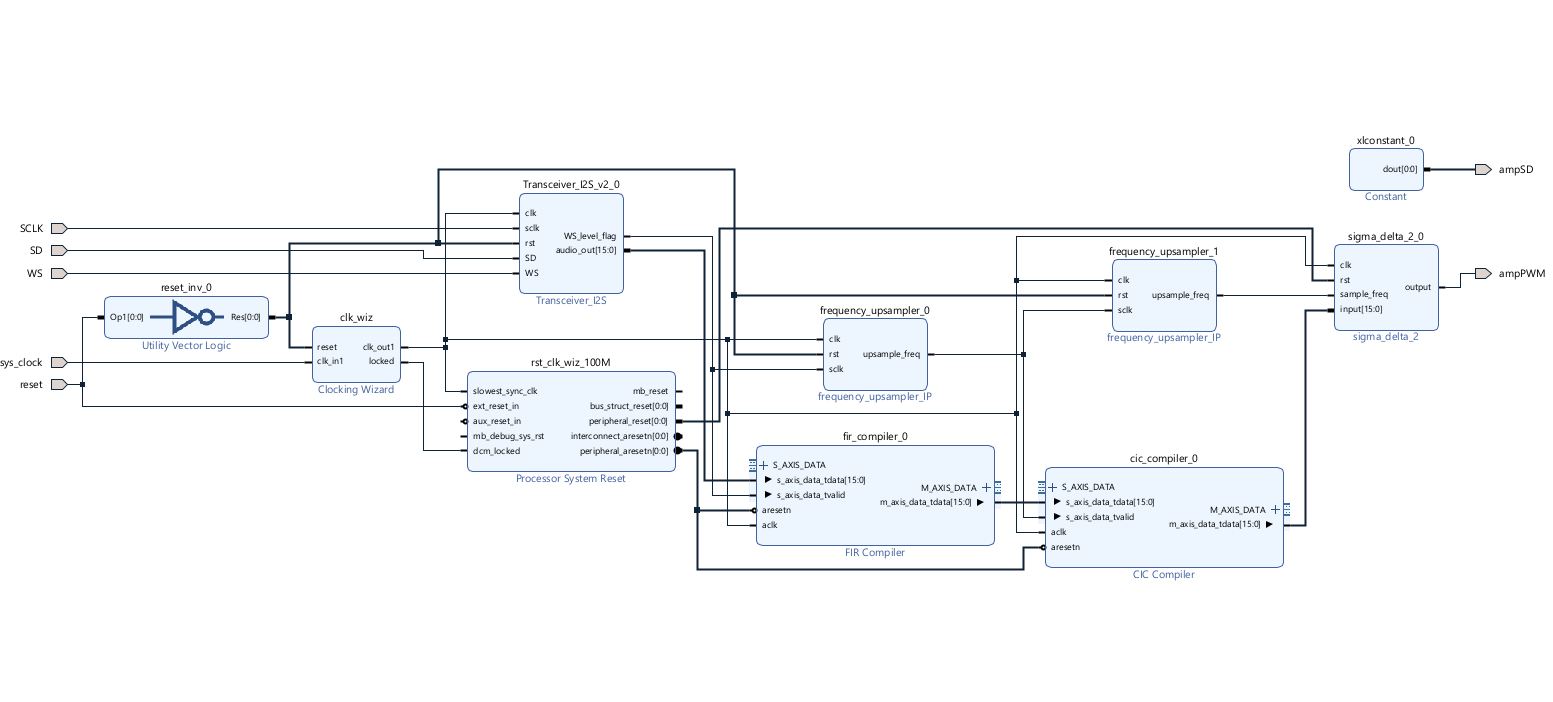
\includegraphics[angle=90,origin=c, width=0.5\linewidth]{Images/VivadoDiagramablocs.png}
    \caption{Diagrama de blocs del projecte al Vivado.}
    \label{fig_VivadoDiagramablocs}
\end{figure}

